\chapter{Implementacija i korisničko sučelje}
		
		
		\section{Korištene tehnologije i alati}
		
			Komunikacija u timu izvedena je putem dva servisa. Korištenjem aplikacije WhatsApp\footnote{https://www.whatsapp.com/}, te na serveru u aplikaciji Discord\footnote{https://discord.com/}. Oboje imaju mogućnosti grupnih poziva, dijeljena ekrana te slanja poruka u grupni \textit{chat}. 
			Za izradu UML dijagrama u dokumentaciji korištena je aplikacija Astah\footnote{https://astah.net/} UML kompanije ChangeVision\footnote{https://www.change-vision.com/}. Za kontrolu verzija izvornog koda korišten je Git\footnote{https://git-scm.com/}, a kao udaljeni repozitorij svog koda i dokumentacije korišten je direktorij na web platformi GitHub\footnote{https://github.com/}.
			Kao razvojno okruženje koristili smo IntelliJ IDEA\footnote{https://www.jetbrains.com/idea/}, integrirano razvojno okruženje (IDE) proizvedeno od strane JetBrains\footnote{https://www.jetbrains.com/}. IntelliJ IDEA koristi se za razvoj aplikacija pisanih u Javi\footnote{https://www.java.com/en/}, Kotlin-u\footnote{https://kotlinlang.org/}, Groovy-u\footnote{https://groovy-lang.org/} i drugim JVM baziranim programskim jezicima.
			Aplikacija je napisana u Java programskom jeziku koristeči alat \textit{Spring Boot}\footnote{https://spring.io/projects/spring-boot/} za razvoj \textit{backenda}, a za razvoj \textit{frontenda} korišten je React\footnote{https://react.dev/}. React je biblioteka programskog jezika JavaScript\footnote{https://www.javascript.com/}, koja se koristi za razvoj programskih sučelja, a stvorio ju je i održava Meta\footnote{https://about.meta.com/}. \textit{Spring Boot} alat je Spring\footnote{https://spring.io/} Framework-a, koji je aplikacijski \textit{framework} za razvoj Java aplikacija, najčešće onih baziranih na rad na web-u.
			Za bazu podataka koristili smo H2\footnote{https://www.h2database.com/html/main.html}, koji je prilagođen radu u Javi i baziran na poslužitelju, za kojeg smo odabrali Render\footnote{https://render.com/}.
			
			\eject 
		
	
		\section{Ispitivanje programskog rješenja}
			
			\textbf{\textit{dio 2. revizije}}\\
			
			 \textit{U ovom poglavlju je potrebno opisati provedbu ispitivanja implementiranih funkcionalnosti na razini komponenti i na razini cijelog sustava s prikazom odabranih ispitnih slučajeva. Studenti trebaju ispitati temeljnu funkcionalnost i rubne uvjete.}
	
			
			\subsection{Ispitivanje komponenti}
			\textit{Potrebno je provesti ispitivanje jedinica (engl. unit testing) nad razredima koji implementiraju temeljne funkcionalnosti. Razraditi \textbf{minimalno 6 ispitnih slučajeva} u kojima će se ispitati redovni slučajevi, rubni uvjeti te izazivanje pogreške (engl. exception throwing). Poželjno je stvoriti i ispitni slučaj koji koristi funkcionalnosti koje nisu implementirane. Potrebno je priložiti izvorni kôd svih ispitnih slučajeva te prikaz rezultata izvođenja ispita u razvojnom okruženju (prolaz/pad ispita). }
			
			
			
			\subsection{Ispitivanje sustava}
			
			 \textit{Potrebno je provesti i opisati ispitivanje sustava koristeći radni okvir Selenium\footnote{\url{https://www.seleniumhq.org/}}. Razraditi \textbf{minimalno 4 ispitna slučaja} u kojima će se ispitati redovni slučajevi, rubni uvjeti te poziv funkcionalnosti koja nije implementirana/izaziva pogrešku kako bi se vidjelo na koji način sustav reagira kada nešto nije u potpunosti ostvareno. Ispitni slučaj se treba sastojati od ulaza (npr. korisničko ime i lozinka), očekivanog izlaza ili rezultata, koraka ispitivanja i dobivenog izlaza ili rezultata.\\ }
			 
			 \textit{Izradu ispitnih slučajeva pomoću radnog okvira Selenium moguće je provesti pomoću jednog od sljedeća dva alata:}
			 \begin{itemize}
			 	\item \textit{dodatak za preglednik \textbf{Selenium IDE} - snimanje korisnikovih akcija radi automatskog ponavljanja ispita	}
			 	\item \textit{\textbf{Selenium WebDriver} - podrška za pisanje ispita u jezicima Java, C\#, PHP koristeći posebno programsko sučelje.}
			 \end{itemize}
		 	\textit{Detalji o korištenju alata Selenium bit će prikazani na posebnom predavanju tijekom semestra.}
			
			\eject 
		
		
		\section{Dijagram razmještaja}
			
			\text Dijagrami razmještaja spadaju pod strukturne i statičke UML dijagrame koji opisuju topologiju sustava, te su usredotočeni na odnos sklopovskih i programskih dijelova. Na slici 5.X prikazan je dijagram razmještaja naše aplikacije. Na klijentskom se računalu nalazi web preglednik kojim se putem HTTPS veze pristupa aplikaciji. Web aplikacija pokrenuta je unutar web poslužitelja, koji se nalazi na poslužiteljskom računalu. Unutar okoline izvođenja web poslužitelja također se nalazi i baza podataka. Razlog manjku zasebnog poslužitelja za bazu podataka je korištenje baze H2, koja je integrirana u \textit{backend}.
			
			%unos slike
			\begin{figure}[H]
				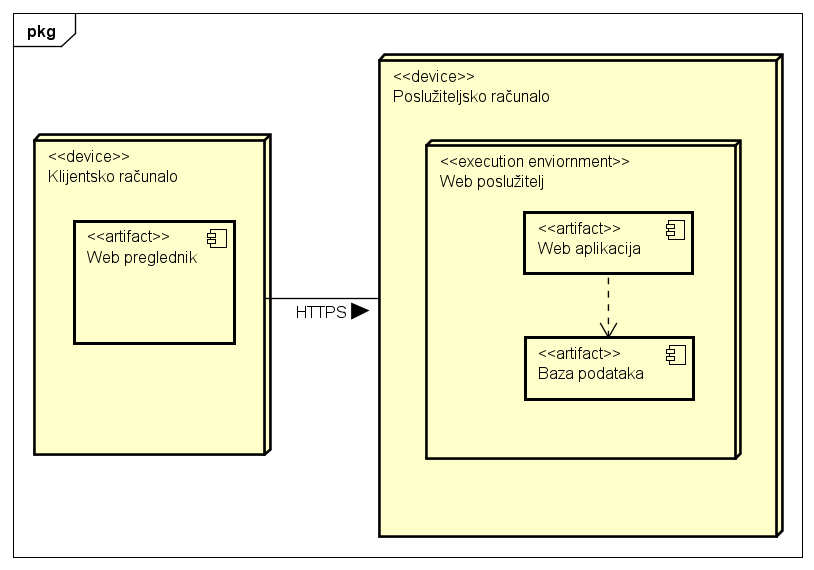
\includegraphics[scale=0.7]{dijagrami/dijrazm1.PNG} %veličina slike u odnosu na originalnu datoteku i pozicija slike
				\centering
				\caption{Dijagram stanja}
				\label{fig:dijstanj1}
			\end{figure}
			
			\eject 
		
		\section{Upute za puštanje u pogon}
		
			\textbf{\textit{dio 2. revizije}}\\
		
			 \textit{U ovom poglavlju potrebno je dati upute za puštanje u pogon (engl. deployment) ostvarene aplikacije. Na primjer, za web aplikacije, opisati postupak kojim se od izvornog kôda dolazi do potpuno postavljene baze podataka i poslužitelja koji odgovara na upite korisnika. Za mobilnu aplikaciju, postupak kojim se aplikacija izgradi, te postavi na neku od trgovina. Za stolnu (engl. desktop) aplikaciju, postupak kojim se aplikacija instalira na računalo. Ukoliko mobilne i stolne aplikacije komuniciraju s poslužiteljem i/ili bazom podataka, opisati i postupak njihovog postavljanja. Pri izradi uputa preporučuje se \textbf{naglasiti korake instalacije uporabom natuknica} te koristiti što je više moguće \textbf{slike ekrana} (engl. screenshots) kako bi upute bile jasne i jednostavne za slijediti.}
			
			
			 \textit{Dovršenu aplikaciju potrebno je pokrenuti na javno dostupnom poslužitelju. Studentima se preporuča korištenje neke od sljedećih besplatnih usluga: \href{https://aws.amazon.com/}{Amazon AWS}, \href{https://azure.microsoft.com/en-us/}{Microsoft Azure} ili \href{https://www.heroku.com/}{Heroku}. Mobilne aplikacije trebaju biti objavljene na F-Droid, Google Play ili Amazon App trgovini.}
			
			
			\eject 